\documentclass[
10pt,
a4paper,
%BCOR=10mm, % boundary correction, lost in binding
bibliography=totoc,
captions=nooneline, % one line caption left aligned just like multiline captions
numbers=noenddot,
twoside]{scrbook}
\addtokomafont{caption}{\small}
\setkomafont{captionlabel}{\sffamily\bfseries}
\setcapindent{0em} % save space with multiline captions; default is \setcaphanging
\setlength{\textheight}{650pt} % keep inner/outer margins, but make text "taller", default 598pt.
\setcounter{secnumdepth}{3}
\setcounter{tocdepth}{3}

\usepackage[T1]{fontenc}
\usepackage[utf8]{inputenc}

% times new roman and matching math font
\usepackage{libertine}
\usepackage{newtxmath}

\usepackage{bm,amssymb,amsfonts,amsmath}  % bold math symbols, AMStex

\usepackage{booktabs}
\usepackage[svgnames]{xcolor}
\usepackage{graphicx}
\usepackage{xspace}
% trailing slash is crucial!
\graphicspath{
  {./}
  {./figures/}
}

\usepackage{hyperref}

\usepackage[numbers,sort&compress]{natbib}
\usepackage{parskip}
\usepackage{marginnote}
\usepackage[colorinlistoftodos]{todonotes} % Use 'disable' to remove todos in final version

\newcommand{\BAT}{{\scshape BAT}\xspace}
\newcommand{\ROOT}{{\scshape ROOT}\xspace}

\newcommand{\BATurl}{http://mpp.mpg.de/bat}
\newcommand{\BATgithub}{https://github.com/bat/bat}
\newcommand{\ROOTurl}{https://root.cern.ch/}

\newcommand{\versionno}{1.1.0-DEV}

\newcommand{\version}{version~\versionno}
\newcommand{\Version}{Version~\versionno}

\newcommand{\code}[1]{\texttt{#1}}

\newcommand{\dan}[1]{{\todo[color=red]{Dan: #1}}}
\newcommand{\fred}[1]{{\todo[color=orange]{Fred: #1}}}
\newcommand{\inbat}[1]{{\todo[color=Salmon!40,inline]{#1}}}
\newcommand{\abstract}[1]{{\todo[color=Grey!40,inline]{#1}}}
\newcommand{\BATnewin}[1]{{\todo[color=Grey!40,noline]{New in v#1}}}
% \newcommand{\BATkeywordsep}[1]{\todo[color=White,noline, bordercolor=White]{\footnotesize \code{#1}}}
\newcommand{\BATkeywordsep}[1]{\marginnote{\footnotesize \code{#1}}}
\newcommand{\BATkeyword}[1]{\code{#1}\BATkeywordsep{#1}}

% references to ...
\def \refchap#1{Chapter~\ref{cha:#1}}
\def \refeq#1{(\ref{eq:#1})}
\def \refsec#1{Section~\ref{sec:#1}}
\def \reffig#1{Figure~\ref{fig:#1}}
\def \reftab#1{Table~\ref{tab:#1}}

% syntax highlighting
\usepackage{listings}
\definecolor{mygray}{rgb}{0.4,0.4,0.4}
\definecolor{mygreen}{rgb}{0,0.8,0.6}
\definecolor{myorange}{rgb}{1.0,0.4,0}
\lstset{
  backgroundcolor=\color{black!5}, % set backgroundcolor
  language=c++,
  gobble=0,
  commentstyle=\itshape\color{purple!80},
  breaklines=true,
  basicstyle=\ttfamily\color{black}\scriptsize,
  frame=single,
  % identifierstyle=\color{blue},
  keywordstyle=\color{myorange},
  numberstyle=\tiny\color{mygray},
  showspaces=false,
  showstringspaces=false,
  stringstyle=\color{myorange},
  tabsize=4,
}
\lstnewenvironment{cxxcode}
{}
{}
\newcommand{\cxxin}[1]{\lstinline{#1}}

% math
\newcommand{\cond}{\,|\,}
\newcommand\rmdx[1]{\mbox{d}#1\,} % differential
\newcommand{\scath}{\theta} % scalar parameter
\newcommand{\vecth}{\bm{\theta}} % vector parameter

% --------------------------------------------------------
% document
% --------------------------------------------------------
\begin{document}

% --------------------------------------------------------
% title
% --------------------------------------------------------

\thispagestyle{empty}

\begin{figure}

\includegraphics[scale=0.25]{bat}
\end{figure}

\vspace*{1cm}

\begin{center}


{\Large \BAT Manual}
\\

\vspace{1cm}

{\large \BAT \version}

\end{center}

\thispagestyle{empty}

\vfill

\begin{center}
\today
\end{center}

\pagebreak

% --------------------------------------------------------
% table of contents
% --------------------------------------------------------

\thispagestyle{empty}

\enlargethispage{2cm}

\tableofcontents{}

% \listoftodos

\mainmatter

\section*{Overview}

The purpose of this document is to introduce the Bayesian Analysis
Toolkit (\BAT), a C++ package providing tools to
\begin{itemize}
  \item compare model predictions with data,
  \item draw conclusions on the validity of a model as a representation of the data,
  \item and to extract the values of the free parameters of a model.
\end{itemize}
For a quick tutorial covering the basic features, jump directly to
\refsec{basics}.

\BAT was originally developed at the \href{http://mpp.mpg.de}{Max
  Planck institute for physics} in Munich, Germany, in the context of
particle physics. \BAT uses \href{\ROOTurl}{\ROOT} for data handling and graphical
output.

\subsection*{Structure of this document}

We give a brief introduction of the Bayesian approach to statistics in
\refsec{Bayes} and describe the core algorithm of \BAT, Markov chain
Monte Carlo, in \refsec{MCMC}. Further sections describe other tools
of \BAT, specific statistical models, and advanced features.

\subsection*{Further help}

Please visit our home page at \url{\BATurl} for an overview of papers,
research, and other activities related to \BAT. The code development
takes place on \href{\BATgithub}{github}.

This document is meant to is quickly enable to you to find your way
around \BAT. We describe the common workflow and explain how to solve
some not-so-common tasks. To keep the size of this document
manageable, we refer to the \href{\BATurl/docs/refman/latest/}{online
  reference guide} in which all classes, methods etc. are documented.

If you run into a problem with \BAT, the preferred method is to create
a new issue on \href{\BATgithub/issues}{github}. This allows other
users to easily find your issue online and benefit from the
solution. If you provide some code for us to reproduce the problem, we
can help you much faster.

For general questions or comments that do not belong into the public
in the form of issues, you can contact the developers at
\href{mailto:bat@mpp.mpg.de}{bat@mpp.mpg.de}.

\part{Basics}
\chapter{Tutorial} \label{sec:basics}

Goal of this section is that you can read and test as you go along, and end up with functioning code.

\section{Installation instructions}

Detailed instructions for downloading and installing BAT are in the
\verb|INSTALL.md| file that comes with the \BAT source distribution. The
latest version is available online at
\url{https://github.com/bat/bat/blob/master/INSTALL.md}.

\fred{Add link to instructions in appendix as per \href{https://github.com/bat/bat/issues/145}{\#145}}

\section{Non-code parts of BAT}
\dan

bat-project, bat-config
\begin{cxxcode}
int main() {
  std::string s = "Hello";
  return 0;
}
\end{cxxcode}

\section{Absolutely necessary requirements of your model}
\dan

Parameters, LogLikelihood, some form of setting a prior.

\section{Running the analysis}
\dan

Functions to call. How to output. Basic tuning. How to interpret runtime log output \& trouble shooting (nonconvergence, poor efficiencies). How to interpret summary log output.

\section{Plots}
\dan

Interpreting the basic output: marginals; parameters; knowledge update; correlation matrix.

Options for the different output types.

\chapter{Bayesian Statistics} \label{sec:Bayes}

In this chapter, we give a concise and necessarily incomplete overview
of Bayesian statistics. Our intention is to cover the bare minimum and
introduce those quantities that appear in \BAT. As a toolkit, \BAT
allows the user complete freedom in modeling. There is vast literature
on the theory, applications, and modeling; for example, consider
\cite{jaynes_probability_2003, hartigan_bayes_1983, sivia_data_2006,
  mackay_information_2003, dagostini_bayesian_2003,
  kendall_kendalls_2004, gelman2014bayesian} for a comprehensive
overview.

\section{Basic terminology} \label{sec:basic-terminology}

Bayesian statistics is a framework for quantitative inductive or
plausible reasoning; i.e., the optimal processing of incomplete
information. The basic idea is to associate a degree of belief to
logical propositions; e.g., the mass of the Higgs boson is 125
GeV. From fundamental axioms about reasoning, one can then show that
the calculus of degree of belief is simply the ordinary calculus of
probability theory; see~\cite{jaynes_probability_2003} for a thorough
discussion. Deductive reasoning is included as the limiting case in
which the degree of belief is either 0 or 1.

From now on, we will use the symbol $P(A)$ to denote both the \emph{degree
of belief} in proposition $A$ and the \emph{probability} of $A$. In our
applications below, $A$ is often one value out of a continuum, so we
use $P(A)$ also to denote the \emph{probability density} of $A$.  The
\emph{conditional probability} of $A$ given $B$ is $P(A \cond B)$.

The two central tasks of the natural sciences are to learn about
nature from data and to make predictions for (future) experiments. A
\emph{model} $M$ is a proxy for all discrete pieces of information relevant
to calculating the degree of belief. The model can contain \emph{parameters}
$\vecth$ that take on values in a continuum, perhaps subject to
constraints as for example $\scath_1 \geq 0$. Bayesian reasoning
provides an update rule to adjust the degree of belief based on new
information available in the form of \emph{observed data} $D$. This update
rule is the celebrated \emph{Bayes' theorem}
\begin{align}
  \label{eq:bayes-thm}
  \boxed{  P(\vecth \cond D, M) \propto P(D|\vecth, M) P(\vecth \cond M)
  }
\end{align}
$P(\vecth \cond M)$ is the \emph{prior density}, $P(D|\vecth, M)$ is
called the \emph{probability of the data} when treated as a function
of $D$, and known as the \emph{likelihood} when considering the
dependence on $\vecth$, for fixed $D$. The model-dependent
normalization constant is known as the \emph{evidence} or
\emph{marginal likelihood}:
\begin{equation}
  \label{eq:evidence}
  Z = \int \rmdx{ \vecth} P(D|\vecth, M) P(\vecth \cond M).
\end{equation}
Finally, the left-hand side of \eqref{eq:bayes-thm}, $P(\vecth | D,
M)$, is the \emph{posterior density}. Prior and posterior (``density''
is usually omitted) represent the state of knowledge about the
parameter $\vecth$ before and after seeing the data. Note that
$\vecth$ appears on opposite sides of ``|'' in $P(D|\vecth,M)$ and
$P(\vecth|D,M)$. That's why Bayes' theorem is also known as the
theorem of \emph{inverse probability}.

\subsection{Marginalization} \label{sec:marginalization}

Suppose there are two parameters, $\vecth = (\scath_1, \scath_2)$, and
$\scath_1$ is the \emph{parameter of interest} whereas $\scath_2$ is a
\emph{nuisance parameter}. In Bayes' theorem, there is no fundamental
distinction between parameters of interest and nuisance parameter,
they are all just parameters. But often the goal of the analysis is to
extract the posterior of $\scath_1$ while $\scath_2$ is only needed at
an intermediate stage; for example in order to correctly model the
measurement process of $D$. From the joint posterior $P(\scath_1,
\scath_2 | D)$, we compute the \emph{marginalized} posterior and can
remove the dependence on $\scath_2$ by integration
\begin{align}
  \label{eq:marginal}
  P(\scath_1 | D) = \int \rmdx{\scath_2} P(\scath_1, \scath_2 | D).
\end{align}

\subsection{Model comparison} \label{sec:model-comparison}

If there is only a single model under consideration, and no potential for
cconfusion, the model label $M$ is implied and usually omitted from the
equations. But suppose that there are two competing models, $M_1, M_2$, with
parameters $\scath_{1,2}$, that quantitatively predict the outcome $D$ of an
experiment. The task is to find the model with the higher degree of
belief. Using Bayes' theorem, the \emph{posterior odds} of the models are easily
found as
\begin{equation}
  \label{eq:post-odds}
  \frac{P(M_1|D)}{P(M_2|D)}
   = B_{12}  \cdot  \frac{P(M_1)}{P(M_2)},
\end{equation}
 where the \emph{Bayes factor} of $M_1$ versus $M_2$, $B_{12}$, is just the ratio
of the evidences
\begin{equation}
  \label{eq:Bayes-factor}
  B_{12}= \dfrac{P(D|M_1)}{P(D|M_2)} = \frac{Z_1}{Z_2}
  = \frac{\int \rmdx{\vecth_1} P(D|\vecth_1, M_1) P(\vecth_1, M_1)}
  {\int \rmdx{ \vecth_2} P(D|\vecth_2, M_2) P(\vecth_2, M_2)}
\end{equation}
The \emph{prior odds} $P(M_1)/P(M_2)$ represent the relative degree of belief
in the models, independent of the data.
% The data are accounted for in the Bayes factor.
The Bayes factor quantifies the relative shift of degree of belief
induced by the data. In general, $\dim \vecth_1 \ne \dim \vecth_2$,
and without loss of generality let $\dim \vecth_1 < \dim
\vecth_2$. The Bayes factor automatically penalizes $M_2$ for its
larger complexity, as the prior mass is spread out over a
higher-dimensional volume. However, this can be compensated if the
likelihood $P(D|\vecth_2, M_2)$ is significantly higher in regions of
reasonably high prior density; i.e. the Bayes factor implements
Occam's razor the simplest model that describes the observations is
preferred.

\section{Goodness of fit} \label{sec:goodness-fit} In the Bayesian
approach, there is, however, no straightforward answer to the
following question: if there is only one model at hand, how to decide
if that model is sufficient to explain the data, or if the search for
a better model needs to continue?  The standard procedure to tackle
this problem of evaluating the \emph{goodness of fit} is to define a
test statistic $T=T(D)$ and to evaluate the following tail-area
probability, that is the $p$ value
\begin{align}
  \label{eq:pvalue}
  p \equiv \int_{T>T_{obs}} \rmdx{T} P(T|M).
\end{align}
Care has to be taken in the usage, computation, and interpretation of
$p$ values. An introduction a Bayesian interpretation of $p$ values
with applications in \BAT is available at \cite{Beaujean:2011zz}; see
also the references therein.

\section{Representation in \BAT} \label{sec:representation-bat}
\fred{The whole section might go somewhere else where users find it more
  easily. I fear it would get lost here}

In \BAT, a model $M$ is represented as a C++ subclass of
\BATkeyword{BCModel}. The crucial parts are to define the likelihood
$P(D \cond \vecth, M)$\BATkeywordsep{LogLikelihood}, the prior
$P(\vecth \cond M)$, and the parameters $\vecth$. From these
quantities, \BAT can compute the posterior $P(\vecth \cond D,
M)$\BATkeywordsep{LogAPrioriProbability}. To avoid numerical overflow,
\BAT operates on the log scale whenever possible.  The key methods of
\code{BCModel} that a user has to implement are
\begin{cxxcode}
virtual double LogLikelihood(const std::vector<double>& params)
virtual double LogAPrioriProbability(const std::vector<double>& params)
\end{cxxcode}
The parameter values are passed in simply as numbers to likelihood and
prior, all parameters are assumed to be real and continuous. Discrete
parameters are not supported. The support of $\vecth$ is a
hyperrectangle whose bounds are given by the bounds of the individual
parameters when added to the model with \BATkeywordsep{AddParameter}
\begin{cxxcode}
bool BCModel::AddParameter(const std::string& name, double min, double max, const std::string& latexname = "", const std::string& unitstring = "")
\end{cxxcode}
The optional \cxxin{latexname} and \cxxin{unitstring} are used only
for labeling plot axes; it's intended usage is to pretty up plots. For
example, a parameter \cxxin{theta} representing a time measured in
seconds is defined as
\begin{cxxcode}
AddParameter("theta", 0, 1, "#theta", "s");
\end{cxxcode}
and whenever \cxxin{theta} appears on the x axis of a plot, it will
appears as ``$\theta$ [s]''. Note that the plots are created with \ROOT,
so the \cxxin{latexname} has to be in \ROOT syntax which is mostly
 \LaTeX{} syntax with ``\textbackslash" $\to$ ``\#''.

\chapter{Markov chain Monte Carlo} \label{sec:MCMC}

\fred{workhorse of BAT. mention Metropolis algorithm, role of proposal function, different choices in bat, why it has to be adapted in prerun. What else happens in prerun:R value and convergence checking. Mention that samples are correlated, chains can get stuck if model wrong/poor.}

\section{Motivation}\label{sec:mcmc-motivation}

The reason that \BAT exists is that nearly any Bayesian analysis
these days is too complicated to be handled analytically. To address
typical questions like
\begin{enumerate}
  \item What is known about a single parameter taking into account
  the uncertainty on all other parameters?
  \item How are parameters correlated?
\end{enumerate}
one needs to be able to compute and visualize 1D and 2D \emph{marginal distributions}; cf. \refsec{marginalization}. These are defined as integrals over the posterior; for  example in 2D
\begin{align}
  \label{eq:mcmc-marginal}
  P(\theta_1, \theta_2 \cond D) = \int \prod_{i \ne 1,2} \rmdx{\theta_i} P(\vecth \cond D).
\end{align}
When the number of parameters grows, the only feasible algorithms to
perform the integration are Monte Carlo methods; i.e., methods based
on random numbers.

The key ingredient in \BAT is an implementation of the Metropolis
algorithm to create a Markov chain; i.e. a sequence of (correlated)
samples from the posterior. We use the shorthand MCMC for Markov chain
Monte Carlo.

\section{Foundations}\label{sec:mcmc-foundations}

Efficient MCMC algorithms are the topic of past and current
research. This section is a concise overview of the general idea and
the algorithms available in \BAT. For a broader overview, we refer the
reader to the abundant literature; e.g., \fred{Robert+Casella, MCMC
  handbook}.

In \BAT, there are several variants of the random-walk Metropolis Hastings algorithm available. The basic idea is captured in the 2D example shown in \reffig{random-walk-idealized}. Given an initial point $x_0$, the Metropolis algorithm produces a sample in each iteration $t=1 \dots$ as follows:

\begin{enumerate}
  \item Propose a new point $y$
  \item Generate a number u from the uniform distribution on [0,1]
  \item Set $x_{t} = y$ if $ u < \frac{P(y \cond D)}{P(x_{t-1} \cond D)}$
  \item Else stay, $x_t = x_{t-1}$
\end{enumerate}

\begin{figure}[ht]
  \centering
  % \includegraphics[width=0.8\textwidth]{random-walk}
  \Large
  \def\svgwidth{1\columnwidth}
  \input{figures/random-walk.pdf_tex}
  \caption{2D random walk. The chain begins in the lower left
    corner. Rejected moves are indicated by the dashed arrow, accepted
    moves are indicated by the solid arrow. The circled number is the
    number of iterations the chain stays at a given point $\vecth = (\theta_1, \theta_2)$.}
  \label{fig:random-walk-idealized}
\end{figure}

\section{Convergence}\label{sec:convergence}
\fred{mixing, burn in, R value, multimodal problems}

\section{Implementation in BAT}

Implementing the Metropolis algorithm, one has to decide on how to
propose a new point based on the current point. For a random walk,
this is given by the \emph{proposal distribution} $q(y \cond x)$. The
main difference between MCMC algorithms is typically given by
different choices of $q$. The Metropolis algorithm doesn't specify
 which $q$ to choose, so we can tune it according to our needs.

In \BAT, the proposal is \emph{symmetric} around the current point
\begin{align}
  q(y \cond x) = q(x \cond y).
\end{align}

There are two stages


\fred{Overall scheme: prerun and main run, adaptation in the prerun}

We offer two variants termed \emph{factorized} and \emph{multivariate}.

\subsection{Factorized proposal}\label{sec:factorized}

\inbat{Factorized was the default and only choice prior to v1.0 and continues to be available.}

\fred{how to activate it}

\abstract{The factorized proposal in $d$ dimensions is a product of 1D
  proposals.}

We sequentially vary one parameter at a time and complete
one iteration of the chain once a new point has been proposed in every
direction. This means the chain attempts to perform a sequence of
axis-aligned moves in one iteration.

\fred{Easiest to understand would be pseudocode}

Each 1D proposal is a Cauchy or Breit-Wigner function centered on the
current point. The scale parameter is adapted in the prerun to achieve
an acceptance rate in a given range that can be adjusted by the
user. Note that there is a separate scale parameter in every dimension.

This means the posterior is called $d$ times in every iteration. Since
the acceptance rate\fred{to define before} is typically different from
zero or one, the factorized proposal typically generates a new point
in every iteration that differs from the previous point in some but
not all dimensions.

\subsection{Multivariate proposal}\label{sec:multivariate}

\BATnewin{1.0} Changing all $d$ parameters at once within one
iteration is an all-or-nothing approach. If the proposed move is
accepted, all parameters have changed for the price of a single
evaluation of the posterior. If the move is rejected, the new point is
identical to the old point and the chain does not explore the
parameter space.

We implement the adaptive algorithm by~\cite{Haario:2001}. In brief,
the proposal is a multivariate Gaussian or Student's t distribution
whose covariance is learned from the covariance of samples in the
prerun. An overall scale factor is tuned to force the acceptance rate
into a certain range.

\fred{Pseudocode}

\subsection{Comparison}\label{sec:proposal-comparison}

Comparing the factorized propoasal to the multivariate proposal, we
generally recommend the multivariate for most purposes. B

Use the factorized proposal if you can speed up the computation of the
posterior if you know that some parameters did not change. This can be
useful if the computation is expensive from some but not all
parameters.

\chapter{Non-MCMC parts of BAT}

\section{Integration}
\fred{Users are confused what integration is needed for: state clearly that cuba is only for evidence. But marginalization can be done by something else than MCMC. We have grid methods implemented}


\section{Optimization}
\fred{afterburner or stand-alone, minuit, simulated annealing. How to get results from Minuit run}

\chapter{Accompanying Models}

\section{Using BAT's native data structures}

\section{base}
\section{Efficiency Fitter}
\section{Graph Fitter}
\section{Histogram Fitter}

\section{mtf}
\fred{Kevin should give advice here. Need channels, processes, goodness of fit}

\pagebreak
\part{Advanced BAT}

\chapter{Structure of the code}
\fred{A few paragraphs, what inherits from what, parameter handling,
  pointer to the reference guide where more info is available such
  that one can click directly on classes etc.}

\chapter{ModelManager for Model Comparison}
\fred{can work on same data set but not required}


\chapter{Defining a factorized prior}

If a model does not overload \code{BCModel::LogAPrioriProbability},
then its prior is the product of the individual priors for each of its
parameters. We call these the factorized priors. To set a parameter's
prior call
\begin{cxxcode}
BCParameter::SetPrior(BCPrior* const prior);
\end{cxxcode}
You can call factorized priors within your overloaded
\code{LogAPrioriProbability} by querying the log of the prior of a
particular parameter with
\begin{cxxcode}
BCParameter::GetLogPrior(double x) const;
\end{cxxcode}

The prior you set for a parameter need only inherit from
\code{BCPrior}. BAT has several built in prior classes, such as
\code{BCConstantPrior} and \code{BCGaussianPrior}.  You can implement
new factorized priors by inheriting from the \code{BCPrior} class. To
illustrate how to do this, we will work through the construction of
the Gaussian prior:
\begin{cxxcode}
class BCGaussianPrior : public BCPrior
\end{cxxcode}
\code{BCPrior} is a pure-virtual class with three methods that must be overloaded:
\begin{cxxcode}
double GetLogPrior(double x);
BCPrior* clone() const;
bool IsValid() const;
\end{cxxcode}
The first one contains the meat of our new prior:
\begin{cxxcode}
double GetLogPrior(double x)
{
  return -0.5 * (x - fMean) * (x - fMean) / fSigma / fSigma - log(fSigma) - 0.5 * log(2 * M_PI);
}
\end{cxxcode}
This is, naturally, the log of a Guassian prior. The second one should
simply return a copy of the prior:
\begin{cxxcode}
BCPrior* clone() const
{
  return new BCGaussianPrior(*this);
}
\end{cxxcode}
The last function is required for checking that everything that is
needed by the prior is properly set. You'll notice that our example
calls on two member variables in its \code{GetLogPrior}: \code{fMean}
and \code{fSigma}. So we must check whether they have been properly set:
\begin{cxxcode}
bool IsValid() const
{
  return std::isfinite(fMean) and std::isfinite(fSigma) and fSigma > 0;
}
\end{cxxcode}
This checks that the mean and standard deviation are both finite and
that the standard deviation is positive semi-definite, as it need be.

Naturally to be of use, we also create a constructor that allows us to
set the mean and standard deviation at creation; and getters and
setters that allow us to access them. (See the source code of
\code{BCGaussianPrior} for their implementation.)

This is all that is required to create a new prior. \code{BCPrior} has
several methods for getting properties of the prior: the mode; the
integral over a range; the $n$'th raw, central, and standardized
moments; the mean; the variance; the standard deviation; the skewness;
and the kurtosis. These functions make their own internal calculations
and need not be overloaded. If you wish to speed them up, or provide
exact results, you may overload them. But take care that you overload
them to give back proper results! For example, the mode of the
Gaussian distribution is not simply \code{fMean}, since this presumes
the range over which we query contains \code{fMean}. The more proper
implementation is
\begin{cxxcode}
double GetMode(double xmin, double xmax)
{
  if (fMean < xmin)
    return xmin;
  if (fMean > xmax)
    return xmax;
  return fMean;
}
\end{cxxcode}

\chapter{Sharing / Loading samples}

You can output the samples of \BAT's Markov chains in the form of a
\ROOT \code{TTree} saved in a \code{TFile}. You can read these samples
back into \BAT using \code{BCEmptyModel}:\footnote{You can also
  use an instance of your model if you provide a constructor that
  calls the \code{BCModel::BCModel(const std::string\& filename, const
    std::string\& name, bool loadObservables)} constructor.}
\begin{cxxcode}
BCEmptyModel m(``MyModel_mcmc.root'');
m.Remarginalize();
\end{cxxcode}
where ``MyModel\_mcmc.root'' is a \code{.root} file produced by a \BAT
analysis---that is, it contains two \code{TTree}'s, ``X\_mcmc.root''
and ``X\_pars.root'', where X is a prefix common to both trees. \BAT
will search the file for two such trees matching the structures
expected from \BAT output. Alternatively, the constructor can be
called with the prefix specified explicitly:
\begin{cxxcode}
  BCEmptyModel::BCEmptyModel(const std::string& filename, const std::string& name, bool loadObservables).
\end{cxxcode}
The last argument tells switches on or off the loading of
\code{BCObservable}'s stored in the \code{TTree}.

Note that instead of calling \code{MarginalizeAll()}, a reloaded \BAT
analysis is marginalized by calling \code{Remarginalize()}.

All subsequent drawing or accessing of \code{BCH1D} and \code{BCH2D}
objects is the same as if the analysis had been run directly rather
than reloaded. For most summary reports of \BAT, the actual model
itself is not needed---only the samples. So you can share your results
by sharing your \ROOT output files without sharing your model
implementation.

Likewise, when outputting to a \ROOT file, \BAT (by default) autosaves
the Markov chains to the ouput file at regular intervals. You can use
the steps outlined above to check the state of an ongoing analysis
using \code{BCEmptyModel}.

\chapter{Uncertainty propagation} \label{cha:uncert-prop}
\fred{How to compute BCObservables, example in ratio model. Plotting of BCObservables, example: 1 parameter changing, evaluate function at 20 points}

\chapter{Performance / Threading / User's attention to thread-safety}

\fred{tips taken over from old manual and expanded. Some advice when it can provide speed up, clearly state that only the MCMC is with threads but synchronization is a bottle neck for fast posteriors}

\chapter{Output}
\section{Logging}
\section{Textual summary}
\fred{summary output, latex tables}
\section{Graphical summary}
\fred{BCSummaryTool}

\chapter{Examples}

\fred{how to run them, suggest to modify them}

\chapter{Validation}

\fred{make check, unit test, performance test suite, building on various platforms}

\chapter{Troubleshooting or FAQ}

\chapter{Tuning MCMC}

\fred{
 scales dimish to zero, chains stuck: error in the model, parameter ranges inappropriate
}

\bibliographystyle{plain}
\bibliography{references.bib}

\end{document}

% Local Variables:
% compile-command:"rubber --pdf --synctex -W refs -W misc manual"
% End:
